\subsubsection*{Pulsaciones}



\item \label{pendacop}
\begin{minipage}[t][2.2cm]{0.75\textwidth}
Considere el sistema de dos péndulos de igual longitud $l$ pero de masas diferentes $m_{a}$ y $m_{b}$, acoplados mediante un resorte
de constante $k$.
\end{minipage}
\begin{minipage}[c][2cm][t]{0.2\textwidth}
  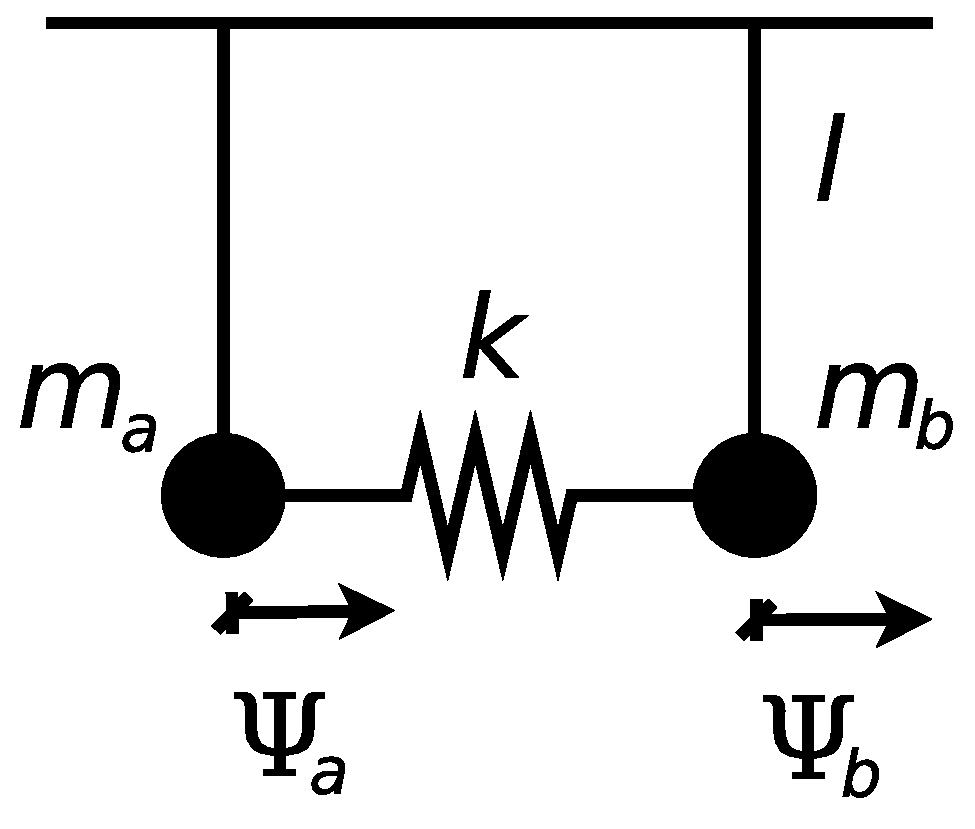
\includegraphics[width=\textwidth]{ej1-7}
\end{minipage}
\begin{enumerate}
	\item Escriba las ecuaciones de movimiento de cada masa. considerando pequeñas oscilaciones, ¿es relevante considerar $l_0\neq0$? ¿Qué cambia si el resorte es \emph{slinky}?   
	\item Obtenga las frecuencias naturales del sistema y sus modos normales de oscilación.
Interprete el significado físico de estos modos normales. 
	\item Suponga que el acoplamiento es débil ($k\ll\frac{g}{l}\frac{m_{a}m_{b}}{m_{a}+m_{b}}$) y que las condiciones iniciales son: $\dot{\Psi}_{a}(0)=0,\dot{\Psi}_{b}(0)=0,\Psi_{a}(0)=0,\Psi_{b}(0)=1$.
Obtenga el movimiento de cada masa y grafíquelo en función del tiempo.
	\item Calcule los valores medios, en un ciclo rápido, de $T_{a}$ y $T_{b}$, donde $T$ indica energía cinética. Grafique $\left\langle T_{a}\right\rangle $ y $\left\langle T_{b}\right\rangle $, y analice las diferencias en el gráfico como función de las diferencias entre las masas ($m_{a}=m_{b}$ y $m_{a}$ muy diferente de $m_{b}$).
Calcule el valor medio de la energía de interacción entre las dos partículas.
\end{enumerate}



\item \label{2masitas}
\begin{minipage}[t][2.8cm]{0.7\textwidth}
Considere el sistema de la figura. Las masas están apoyadas en una mesa sin rozamiento, sujetas a las paredes por resortes de constante
$k$ y unidas por otro resorte de constante $k'$.
\begin{enumerate}
	\item Obtenga las frecuencias y los modos transversales del sistema. 
	\item ¿Bajo qué condiciones espera observar batidos?
	¿Qué son los batidos?
\end{enumerate}
\end{minipage}
\begin{minipage}[c][0cm][t]{0.25\textwidth}
  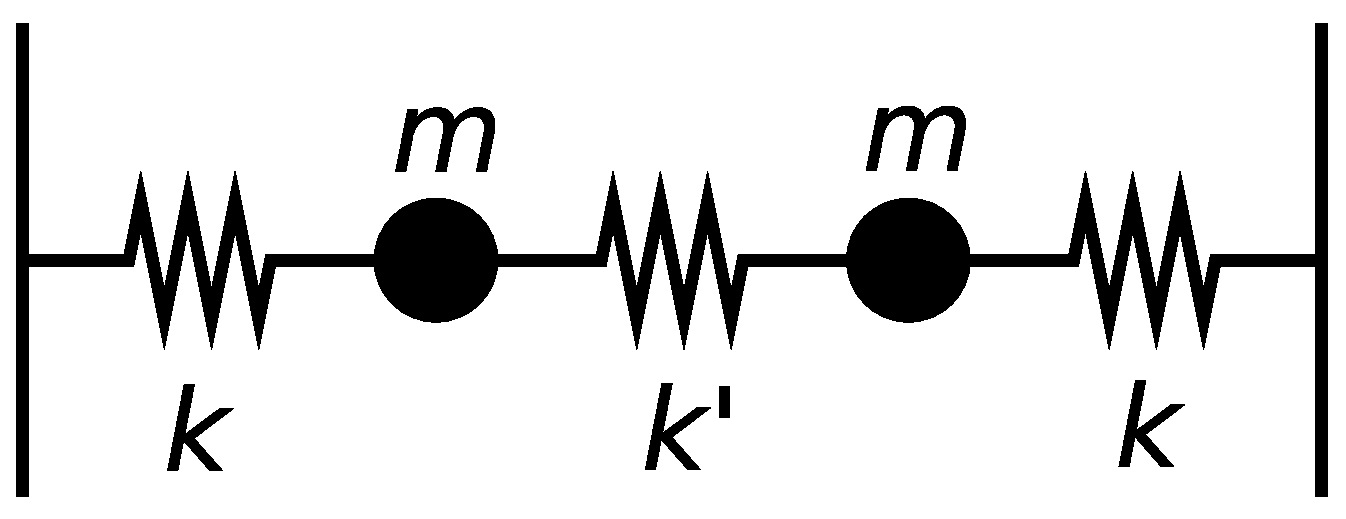
\includegraphics[width=\textwidth]{ej1-8}
\end{minipage}


